\documentclass[11pt,letterpaper]{article}
\usepackage{fcfm}

\begin{document}

%------ Header -------- %
\customheader{Operations Research}{Group: 032}{The Use of \textit{"Lorem Ipsum"} in \LaTeX{} Templates}{October 14, 1582}

\rule{17cm}{0.1mm}

\authorrowthree
  {\customauthor{Albert Einstein}{aeinstein@princeton.edu}{Institute for Advanced Study}{Princeton, New Jersey, USA}}
  {\customauthor{Marie Curie}{mcurie@sorbonne.fr}{Université de Paris}{Paris, Île-de-France, France}}
  {\customauthor{Isaac Newton}{inewton@cam.ac.uk}{University of Cambridge}{Cambridge, England, UK}}

\authorrowtwo
  {\customauthor{Galileo Galilei}{ggalilei@unipi.it}{Università di Pisa}{Pisa, Tuscany, Italy}}
  {\customauthor{Charles Darwin}{cdarwin@cam.ac.uk}{University of Cambridge}{Downe, Kent, England, UK}}

\authorrowone
  {\customauthor{Luis A. Gutierrez-Rodriguez}{lgutierrezr@uanl.edu.mx}{Universidad Autónoma de Nuevo León}{San Nicolás de los Garza, Nuevo León, MX}}

\rule{17cm}{0.1mm}

\begin{abstract}
Rummikub is a popular tile-based game that involves both combinatorial optimization 
and strategic decision-making. This paper presents a formal investigation into the game 
mechanics, identifies the core computational challenges, and introduces an integer 
programming (IP) model designed to find optimal moves for a given player state. 
We analyze the problem space, define constraints based on legal game rules, and 
propose an IP formulation to maximize score per turn. Giving a future insight into 
applying possible Counting strategies to optimize decision making when given 
multiple players' states.
\end{abstract}

\smallskip
\noindent\textbf{Keywords:} \LaTeX{}, Lorem Ipsum, lipsum, templates, document formatting, placeholder text, typography.

\section*{Introduction}
Rummikub is a widely played tile-based game that combines elements of rummy and mahjong. 
Players aim to be the first to empty their racks by forming sets and runs using numbered 
and colored tiles. While the rules are simple, the combinatorial complexity that emerges 
as the game progresses makes decision-making increasingly difficult. A player may have 
many possible ways to arrange their tiles on the board, particularly when they are allowed 
to manipulate existing sets. Deciding on the best possible move—i.e., the one that maximizes 
the number or value of tiles placed on the table—is a non-trivial problem.

In this research, we investigate the use of Integer Linear Programming (ILP) to solve the 
Rummikub move optimization problem. Our goal is to develop a mathematical model that, given 
a current board state and a player's hand, determines the optimal set of tile moves that 
obey all Rummikub rules while maximizing a strategic objective, such as the number or 
value of tiles placed. This approach is based on the successful work of Den Hertog and 
Hulshof (2006), who showed that Rummikub configurations can be effectively modeled and 
solved using ILP within seconds, even in nontrivial game states.

\subsection*{Why use Integer Linear Programming?}
Integer Linear Programming is a branch of mathematical optimization used for solving decision
problems involving discrete variables and linear relationships. In ILP, the goal is to 
maximize or minimize a linear objective function (like total tile value placed), subject 
to a set of linear equality or inequality constraints (like the legal formation of sets).

In Rummikub, each decision—whether to play a tile, form a group or a run, or manipulate the 
board—can be encoded as a binary or integer variable (e.g., "1" if the tile is used, "0" if 
not). The constraints ensure that moves are legal according to the game rules (e.g., sets 
must contain valid combinations of numbers and colors, no tile can be used more than once, 
jokers are used properly, etc.).

Using ILP offers several advantages:
\begin{itemize}
    \item Optimality: It guarantees the best move given the current information.

    \item Flexibility: Complex rules (like joker usage and minimizing board changes) can be incorporated as constraints or secondary objectives.

    \item Speed: With modern solvers, even complex configurations can be solved in under a second.

\end{itemize}
This is especially valuable in Rummikub because brute-force enumeration of all legal move 
combinations becomes computationally infeasible as the number of tiles increases. We will further
explore the brute-force enumeration search space, when discussing the ILP model.

\section*{Background Game Rules and Complexity}
\subsection*{Rummikub Game Rules Overview}
Rummikub is a tile-based game for 2 to 4 players (or up to 6 with extended sets). The goal is to be the first to eliminate all tiles from one's rack by forming valid sets according to specific rules. Below, we summarize the essential components and gameplay mechanics relevant to our mathematical modeling.

\subsection*{Objective}
The aim of the game is to place all the tiles from one's rack onto the table by forming valid sets: \textbf{groups} or \textbf{runs}.

\subsection*{Tile Set}
The complete game includes:
\begin{itemize}
    \item 106 tiles: two sets of tiles numbered 1 to 13 in four colors (red, blue, black, and orange), plus 2 jokers.
    \item Each player starts with 14 tiles on a personal rack.
    \item Remaining tiles form a face-down pool.
\end{itemize}

\subsection*{Valid Sets}
\begin{itemize}
    \item \textbf{Group:} Three or four tiles of the same number in different colors.
    \item \textbf{Run:} Three or more consecutive numbers in the same color.
\end{itemize}

\subsection*{Setup}
\begin{itemize}
    \item Players draw one tile each; the highest goes first.
    \item All tiles are then shuffled and stacked in piles (optional for convenience).
    \item Each player draws 14 tiles for their rack.
\end{itemize}

\subsection*{Initial Meld}
\begin{itemize}
    \item A player's first move must consist of one or more valid sets with a combined value of at least 30 points.
    \item Tiles used must come solely from the player’s rack.
    \item Jokers may be used and are valued as the tile they represent.
    \item If unable or unwilling to make the initial meld, the player draws a tile from the pool and ends their turn.
\end{itemize}

\subsection*{Gameplay}
\begin{itemize}
    \item Turns proceed clockwise.
    \item After the initial meld, players may:
    \begin{itemize}
        \item Add tiles to existing sets on the table.
        \item Rearrange existing sets (manipulation) to create new valid sets.
    \end{itemize}
    \item If no valid move is possible, the player must draw a tile and end their turn.
    \item Tiles drawn cannot be played until the player's next turn.
\end{itemize}

\subsection*{Manipulation Rules}
Players may manipulate sets on the table under the following conditions:
\begin{itemize}
    \item At the end of the turn, all tiles on the table must be in valid sets.
    \item No tiles may remain loose or isolated.
    \item Jokers may be replaced if the player can substitute them with the correct tile.
    \item The joker must then be immediately reused to form a new set in the same turn.
\end{itemize}

\subsection*{The Joker}
\begin{itemize}
    \item Acts as a substitute for any tile in a valid set.
    \item Can be reclaimed if replaced by the tile it represents.
    \item Must be played immediately in a new set using at least one tile from the player’s rack.
    \item Cannot be used before the player's initial meld is completed.
\end{itemize}

\subsection*{Winning and Scoring}
\begin{itemize}
    \item A game ends when a player empties their rack.
    \item Other players total the value of the tiles remaining on their racks; this becomes their negative score.
    \item The winner scores the sum of the other players’ negative scores as a positive amount.
    \item The joker carries a penalty of 30 points if left on a rack.
    \item If no player can make a move and the pool is empty, the player with the lowest rack total wins.
\end{itemize}

\subsection*{Computational Complexity}

The computational complexity of determining an optimal or even a valid move in \textit{Rummikub} has been studied formally. Previous research establishes that the problem of finding a valid move in a generalized version of Rummikub is \textbf{NP-complete}, particularly when the number of tile values and the number of suits are considered as part of the input~\cite{rummikub_complexity}. This complexity arises from the vast number of permutations and combinations that must be evaluated to check whether a selection of tiles can be rearranged into valid sets (runs or groups) under the game’s constraints.

In their work, Bodlaender et al.~\cite{rummikub_complexity} formalize a generalized version of Rummikub, where the number of values $n$, the number of suits $k$, and the number of tile copies $m$ are not fixed, but are instead part of the input. They show that even determining whether a move is valid—i.e., whether a given set of tiles can be partitioned into valid groups and runs—is computationally difficult. The NP-completeness result follows from a reduction from known NP-complete problems, such as the \textsc{3-Partition} problem, leveraging the fact that the constraints in Rummikub closely resemble those involved in such problems.

Moreover, although the decision problem is NP-complete in the generalized setting, the paper also presents a pseudo-polynomial time algorithm when certain parameters are fixed. Specifically, if the number of suits $k$, the number of tile copies $m$, and the group size $s$ are fixed constants, then the problem becomes tractable and can be solved in polynomial time with respect to the number of values $n$. 

This result is particularly relevant to the standard version of Rummikub as played in practice, where these parameters are indeed constants. Thus, while the general case is intractable, there is an important distinction: under fixed parameters (as in real-world games), finding valid moves is computationally feasible. This duality between theoretical complexity and practical playability motivates further algorithmic strategies that exploit these fixed constraints, such as dynamic programming or integer linear programming approaches.


\section*{Problem Definition and Set Enumeration}

\subsection*{Since the Problem We Are Solving}

The core decision-making challenge in a game of Rummikub is determining the best possible move during a player's turn. Specifically, the question is:

\begin{quote}
    \emph{What is the largest number (or total value) of tiles that a player can legally place on the table in a single turn, either by forming new sets or by manipulating existing sets, in accordance with all Rummikub rules?}
\end{quote}

This is a nontrivial problem due to the combinatorial explosion of possible tile groupings and manipulations. A single rack of 14 tiles, combined with the dynamic state of the board, can result in thousands of possible legal moves. Attempting to evaluate all possible combinations by hand or brute-force computation is computationally infeasible. Thus, the use of \textbf{Integer Linear Programming (ILP)} offers a structured way to model these constraints and systematically identify optimal solutions.

To build such a model, it is essential to first define the full universe of legal \textbf{Rummikub sets} (i.e., all combinations of tiles that can be legally played), which is where the number \textbf{1174} plays a critical role.

\subsection*{Enumeration of All Valid Sets}

In Rummikub, a \textbf{set} is a valid grouping of tiles that satisfies one of the following two rules:
\begin{itemize}
    \item \textbf{Group:} Three or four tiles of the same number in different colors.
    \item \textbf{Run:} Three to five\footnote{Note that a run with six or more 
    consecutive numbers can be divided into runs of length three, four or five, and
     so we do not need to consider them seperately} consecutive numbers in the same color.
\end{itemize}

The authors of the original model compute the total number of valid sets that can occur in the game---whether made purely from natural tiles or involving jokers. This total comes out to exactly \textbf{1174 sets} \cite{den2006solving}. Below, we explain how this number is derived.

\subsubsection*{1. Sets Without Jokers}

\begin{itemize}
    \item \textbf{Runs (same color, consecutive numbers):}
    \begin{itemize}
        \item Each color (4 in total) allows for:
        \begin{itemize}
            \item 11 runs of 3 numbers (e.g., 1--3, 2--4, ..., 11--13)
            \item 10 runs of 4 numbers
            \item 9 runs of 5 numbers
        \end{itemize}
        \item Total runs without jokers: $44 + 40 + 36 = 120$
    \end{itemize}

    \item \textbf{Groups (same number, different colors):}
    \begin{itemize}
        \item For each number from 1 to 13:
        \begin{itemize}
            \item Choose 3 out of 4 colors: $\binom{4}{3} = 4$ combinations → $13 \times 4 = 52$
            \item Or all 4 colors → 13 combinations
        \end{itemize}
        \item Total groups without jokers: $52 + 13 = 65$
    \end{itemize}
\end{itemize}

\subsubsection*{2. Sets With Jokers}

Jokers can substitute for any missing tile in a group or run, significantly increasing the number of possible valid sets. The authors enumerated all legal joker-containing combinations by hand and through exhaustive generation, ensuring no illegal duplications.

\begin{itemize}
    \item \textbf{With one joker:}
    \begin{itemize}
        \item 92 valid 3-tile runs
        \item 124 valid 4-tile runs
        \item 148 valid 5-tile runs
        \item 78 valid 3-tile groups
        \item 52 valid 4-tile groups
        \item Total: $92 + 124 + 148 + 78 + 52 = 494$
    \end{itemize}

    \item \textbf{With two jokers:}
    \begin{itemize}
        \item 52 valid 3-tile runs
        \item 132 valid 4-tile runs
        \item 233 valid 5-tile runs
        \item 78 valid 4-tile groups
        \item Total: $52 + 132 + 233 + 78 = 495$
    \end{itemize}
\end{itemize}

\subsubsection*{3. Final Total}

The total number of valid Rummikub sets across all cases is:

\[
\text{No jokers: } 185 \quad + \quad \text{1 joker: } 494 \quad + \quad \text{2 jokers: } 495 \quad = \boxed{1174 \text{ sets}}
\]

These 1174 sets become the foundation of the model: the optimization process selects which sets (from this pool) to use to maximize tile usage on a given turn.

\subsection{Why This Enumeration Matters}

Each set is assigned an index ($j \in \{1, \dots, 1174\}$) and is represented in the ILP model using binary or integer variables. By precomputing the entire universe of legal sets, the model transforms the abstract problem of Rummikub tile play into a structured selection problem with known components, enabling the solver to:
\begin{itemize}
    \item Decide which sets to form (and how many times),
    \item Ensure all tiles are used legally,
    \item Maximize the number (or value) of tiles placed,
    \item Optionally minimize unnecessary changes to the table.
\end{itemize}

\section*{Model Details}

\subsection*{Overview}

To determine the optimal move in a given Rummikub configuration, Den Hertog and Hulshof proposed an Integer Linear Programming (ILP) model. The model computes the best possible placement of tiles from a player’s rack onto the table involving manipulation of existing sets. The optimization goal is to:
\begin{itemize}
    \item Maximize the \textbf{value of tiles} placed (i.e., sum of tile numbers) and minimize unnecessary changes to the table.
\end{itemize}

\subsection*{Model Structure}

The model defines the following sets, parameters, and variables:

\paragraph{Indices:}
\begin{itemize}
    \item $i \in I = \{1, \dots, 53\}$: index for tile types (including the joker).
    \item $j \in J = \{1, \dots, 1174\}$: index for all possible valid sets (runs and groups, with or without jokers).
\end{itemize}

\paragraph{Parameters:}
\begin{itemize}
    \item $s_{ij}$: equals 1 if tile $i$ is part of set $j$; 0 otherwise.
    \item $t_i$: number of times tile $i$ is currently on the table.
    \item $r_i$: number of times tile $i$ is available in the player’s rack.
    \item $v_i$: value of tile $i$ (equal to its number; joker has value of 30 when in player's rack).
    \item $w_j$: number of times set $j$ is currently on the table (for change minimization).
    \item $M$: large constant used to scale the influence of secondary objective (e.g., 40).
\end{itemize}

\paragraph{Variables:}
\begin{itemize}
    \item $x_j \in \{0, 1, 2\}$: number of times set $j$ is formed in the new solution.
    \item $y_i \in \{0, 1, 2\}$: number of times tile $i$ is played from the player’s rack.
    \item $z_j \in \{0, 1, 2\}$: number of times set $j$ appears both in the original table and in the new solution.
\end{itemize}

\subsection*{Objective Function}

\paragraph{Option 1: Maximize number of tiles placed}
\[
\max \sum_{i \in I} y_i
\]

\paragraph{Option 2: Maximize total value of tiles placed}
\[
\max \sum_{i \in I} v_i \cdot y_i
\]

\paragraph{Option 3: Maximize value and minimize changes (model used)}
\[
\max \left( \sum_{i \in I} v_i \cdot y_i + \frac{1}{M} \sum_{j \in J} z_j \right)
\]
The second term rewards preserving existing sets from the original configuration, weighted to be less important than the main objective.

\subsection*{Constraints}

\paragraph{Tile Conservation Constraint:}
\[
\sum_{j \in J} s_{ij} x_j = t_i + y_i \quad \forall i \in I
\]
Each tile used in the final solution must either:
\begin{itemize}
    \item Already exist on the table, or
    \item Be added from the player’s rack.
\end{itemize}

\paragraph{Rack Availability Constraint:}
\[
y_i \leq r_i \quad \forall i \in I
\]
A tile cannot be played more times than it is available in the player’s rack.

\paragraph{Set Preservation Constraints:}
\[
z_j \leq x_j \quad \forall j \in J
\]
\[
z_j \leq w_j \quad \forall j \in J
\]
These ensure that $z_j = \min(x_j, w_j)$ — a set is only considered preserved if it appears both in the original and new table states.

\paragraph{Joker Usage Constraint:}
\[
\sum_{j \in J} s_{\text{joker}, j} \cdot x_j \leq r_{\text{joker}}
\]
This limits the number of jokers used in selected sets to the number available on the player’s rack.

\paragraph{Variable Domains:}
\[
x_j \in \{0, 1, 2\}, \quad y_i \in \{0, 1, 2\}, \quad z_j \in \{0, 1, 2\}
\]

\subsection*{Full Constraint Summary}
\begin{align*}
\sum_{j \in J} s_{ij} x_j &= t_i + y_i &&\forall i \in I \\
y_i &\leq r_i &&\forall i \in I \\
z_j &\leq x_j &&\forall j \in J \\
z_j &\leq w_j &&\forall j \in J \\
\sum_{j \in J} s_{\text{joker}, j} \cdot x_j &\leq r_{\text{joker}} &&\text{(joker limit)} \\
x_j, y_i, z_j &\in \{0, 1, 2\} &&\forall j \in J, i \in I
\end{align*}


\section*{Implementation and Experiments}
\subsection*{Tools Used}
Model implemented using Python and solved with Google OR-Tools\cite{or_tools}.

\subsection*{Test Cases}
Present example game states and corresponding optimal plays derived from the model.


\begin{figure}[h]
    \centering
    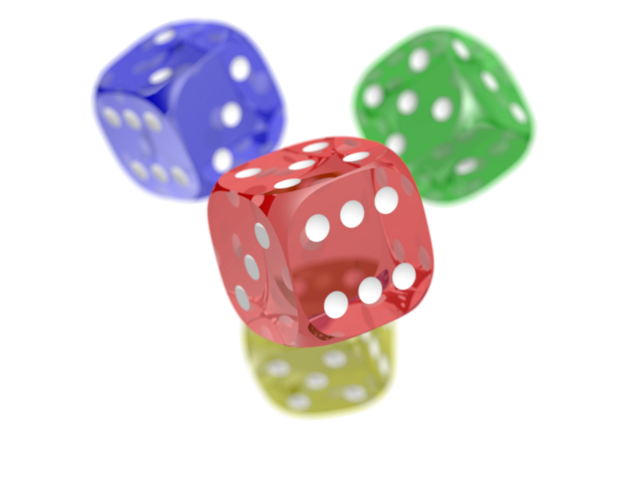
\includegraphics[width=0.7\textwidth]{Figures/example_image.png}
    \caption{Example board configuration solved by the model.}
\end{figure}

\subsection*{Results}
Show performance in terms of solution time, and move quality.

\section*{Discussion}

\subsection*{Limitations}

While the proposed Integer Linear Programming (ILP) model offers a powerful approach for determining optimal Rummikub moves from a static board configuration, several limitations emerged during development and testing.

One major limitation lies in the scalability of the model as board complexity increases. Although the enumeration of all 1174 valid sets provides a comprehensive basis for optimization, the number of possible combinations that need to be evaluated grows significantly when the board contains many pre-existing sets and the player’s rack includes numerous interaction possibilities. This issue becomes more pronounced when considering manipulation of existing sets, which introduces additional layers of complexity and constraint handling. As a result, while our model performs well for moderately complex configurations, its computational efficiency may degrade in scenarios involving deeply interwoven board states or multiple jokers.

Another notable challenge is the handling of dynamic player interaction across turns. The current model assumes a static board and evaluates optimal moves from the perspective of a single player on a single turn. However, Rummikub is inherently a multi-agent game where each player’s action influences the next, potentially invalidating or modifying previously optimal moves. Our framework does not yet accommodate strategic anticipation or planning across multiple turns, nor does it incorporate opponent modeling, bluffing strategies, or risk assessment, all of which are critical components of human-level gameplay.

Moreover, while our code implementation using Google OR-Tools successfully solves the ILP formulation for various static scenarios, it lacks automation in test case generation and does not currently simulate full game progression. Each test must be manually crafted, which limits the breadth and depth of experimentation. The system also cannot yet play multiple turns in sequence or simulate a complete game involving multiple players with evolving board states.

\subsection*{Future Work}

There are several directions for future research and development that could enhance the capabilities and applicability of this model.

First, integrating the ILP solver with other forms of artificial intelligence, such as heuristic search or game-tree evaluation agents, could significantly improve decision-making in more dynamic contexts. A hybrid architecture that combines rule-based pruning with optimization-based planning may be better suited to handle the fluid nature of Rummikub gameplay.

Second, the application of reinforcement learning (RL) represents a promising avenue. An RL agent trained over thousands of simulated games could learn policies that not only evaluate immediate payoff but also account for long-term positioning and strategic manipulation. Reinforcement learning could also guide the agent in choosing between alternative optimal moves when multiple valid solutions exist, based on prior game outcomes or opponent behavior.

Third, one intriguing area to explore is the implementation of \textbf{counting strategies}—techniques commonly used by expert players to track tile frequencies and infer opponents’ likely racks. By embedding probabilistic models into the optimization framework, it may be possible to refine decision-making based on partial information and simulate more intelligent behavior. 

These models would need to balance the computational cost of probabilistic inference with the speed and precision required for real-time gameplay.

Additionally, automating the generation of test scenarios and enabling the simulation of full multi-turn games with multiple players would provide a more robust platform for experimentation. Such a system would allow for comprehensive benchmarking, stress testing of the model under extreme configurations, and the ability to evaluate long-term strategy performance.

Finally, enabling the system to track game progression, adapt to previous moves, and refine its strategy over time would be essential for constructing a competitive AI capable of playing Rummikub autonomously and at a high level.


\section*{Conclusions}
In this work, we have presented a comprehensive mathematical framework for solving the Rummikub move optimization problem using Integer Linear Programming. By defining all 1174 valid tile sets and encoding game rules into a set of linear constraints, we developed a model capable of determining the optimal move for a given player in a static game state. Our ILP model was implemented using Google OR-Tools, and we demonstrated its ability to solve a variety of board configurations effectively, providing optimal solutions that respect all game constraints.

The key strength of our approach lies in its precision and formal rigor. Unlike heuristic or greedy methods, our ILP formulation guarantees the identification of a globally optimal move under the defined objective function—either maximizing the number or total value of tiles placed. Furthermore, the modular nature of the model allows for extensions, such as alternative scoring schemes, secondary objectives (e.g., minimizing board changes), and the inclusion of joker-handling rules.
Nevertheless, the research highlights several challenges that remain to be addressed. The current model operates under the assumption of a single-turn scenario and does not incorporate full game progression or interactions among multiple players. Additionally, the manual nature of test case generation limits the scalability and generalizability of our testing procedures.

Looking ahead, this work lays the foundation for the development of a fully autonomous Rummikub-playing agent. With future enhancements—such as integration with reinforcement learning, dynamic simulation, and probabilistic reasoning—our model could evolve into a sophisticated decision-making engine capable of real-time gameplay. Such an agent could not only serve as a benchmark opponent for human players but also contribute to broader research on optimization and AI in combinatorial games.

In summary, this investigation provides a strong first step toward the automation of intelligent gameplay in Rummikub through mathematical modeling. The fusion of combinatorial enumeration, integer programming, and AI techniques offers a promising pathway to mastering the intricate strategies of this deceptively complex game.

\bigskip

\bibliographystyle{apalike-ejor}
\bibliography{references}

\end{document}
